\section{Introduction}
	The 8-Puzzle is made of 9 squares fashioned in a $3x3$ manner that consists of 8 pieces of tiles that needs to be ordered in such a way that each of the 8 pieces must be placed in its proper place in the $3x3$ board. With 9 squares and 8 pieces, there will be a free space. The challenge for the 8-Puzzle is that the pieces cannot be lifted but can only moved in a ``slide" action. To make an efficient approach for the puzzle, the point of view for searching for the solution to the puzzle is that the free space is considered as the ``moving piece". With this, there would exist four possible actions each movement: north movement, south movement, west movement and east movement of the free space. \cite{back1}

\section{Methodology}
	For solving the 8-Puzzles in this case, Heuristic Algorithms will be used. The algorithms' job is to find the most promising part of the search tree by making use of the information that can be gathered from the domain of the problem.

	\subsection{Search Tree}
		It was discussed above that the free space is the one considered as the ``moving piece" so as to simplify and make efficient the process of searching for the solution to a particular 8-Puzzle Problem. The free space can either move north, south, east or west. For every change in the free space's place, this represents a state node in the search tree. For the search tree of the 8-Puzzle, a node in the search tree represents a possible solution and an edge represents the allowable moves of the free space. Therefore, the graph of solvable 8-Puzzles has $182440$ vertices and $241920$ edges. \cite{back2}
	
	\subsection{The Three 8-Puzzle Solving Algorithms}
		Two most commonly used heuristics for the 8-Puzzle involve counting the number of misplaced tiles (Hamming Heuristic) and finding the sum of the Manhattan distances between each block and its goal position (Manhattan Heuristic). To further explain the two heuristics, the goal state shown in Figure \ref{fig:gs} will be used.
		\begin{figure}[h]
		\centering
		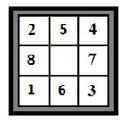
\includegraphics[width=0.18\textwidth]{fig1.jpg}
		\caption{Sample Goal State}
		\label{fig:gs}
		\end{figure}

		\subsubsection{Hamming Function}
			The Hamming heuristic makes use of the number of misplaced tiles for computing the Hamming Function $h_H$. The Hamming function is computed by simply incrementing 1 in every tile that is not in the goal state. A demonstration on how to get the Hamming function is shown in Figure \ref{fig:hamf}.
			\begin{figure}[h]
			\centering
			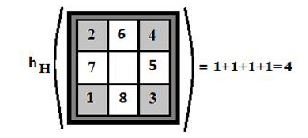
\includegraphics[width=0.4\textwidth]{fig2.jpg}
			\caption{Hamming Function computation}
			\label{fig:hamf}
			\end{figure}

			The Hamming Function implemented in Java is shown at Figure \ref{fig:ham}
			\begin{figure}[h]
			\centering
			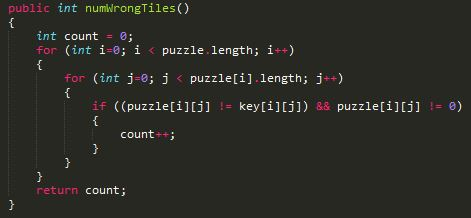
\includegraphics[width=0.4\textwidth]{ham_func.jpg}
			\caption{Hamming Function implementation in Java}
			\label{fig:ham}
			\end{figure}

		\subsubsection{Manhattan Function}
			The Manhattan heuristic uses the summation of each tiles' Manhattan distance for computing the Manhattan Function $h_M$. The Manhattan function is calculated as:
			\begin{equation}
			h_M(S) = \sum ManhattanDistance(k)
			\end{equation}
			where $k \in \lbrace 1,2,...,7,8 \rbrace$ since there are 8 tiles for the 8-Puzzle. $ManhattanDistance(k)$ is then calculated as:
			\begin{equation}
			ManhattanDistance(k) = |x_k - x_{kg}| + |y_k - y_{kg}|
			\end{equation}
			where $x_k$ and $x_{kg}$ is the horizontal distance between a particular tile $k$ to its goal position and $y_k$ and $y_{kg}$ is the vertical distance between a particular tile $k$ to its goal position. Thus $(x_k,y_k)$ is the coordinates of a particular tile $k$ and its goal position is $(x_{kg},y_{kg})$. A demonstration on how to get the Manhattan Function is shown in Figure \ref{fig:manf}.
			\begin{figure}[h]
			\centering
			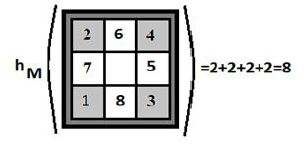
\includegraphics[width=0.4\textwidth]{fig3.jpg}
			\caption{Manhattan Function computation}
			\label{fig:manf}
			\end{figure}

			The Manhattan Function implemented in Java is shown at Figure \ref{fig:man}
			\begin{figure}[h]
			\centering
			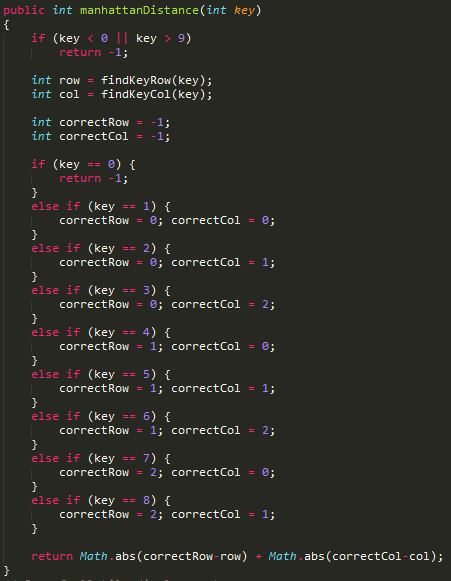
\includegraphics[width=0.4\textwidth]{man_func.jpg}
			\caption{Manhattan Function implementation in Java}
			\label{fig:man}
			\end{figure}

		\subsubsection{Breadth-first Search}
			The Breadth First Search, unlike the two procedures stated above, is a blind search algorithm. Hence, this kind of approach does not use any heuristics since it does not behave based on the state of the problem since it simply traversing the whole search tree until it finds the goal state. This is used so that the differences of blind search and heuristics for this kind of problem would be observed.

\section{Results and Discussions}
	The program was run in an Asus laptop running Windows 10 Home Single Language with system specs shown below:
	\begin{center}
	\textbf{System Specifications}\\
	\begin{tabular}{ |c|c| } 
	\hline
	Processor & Intel(R) Celeron(R) CPU N2940 at $1.83$GHz \\
	\hline
	Installed Memory(RAM) & $4.00$GB ($3.89$GB usable) \\
	\hline
	System type & $64$-bit Operating System, x$64$ based processor \\
	\hline
	\end{tabular} \\
	\end{center}
	After running 10 trials on each of the three 8-Puzzle solving algorithms, the runtimes were gathered and are averaged. Each trial and each solver has used only one randomized initial configuration so as to ensure a consistent and reliable data. The results yielded are as follows:
	\begin{center}
	\textbf{Hamming Heuristic}\\
	\begin{tabular}{ |c|c| } 
	\hline
	Trial & Runtime(ms) \\
	\hline
	\multirow{1}{3em}{1st}
	& 6149 \\
	\hline
	\multirow{1}{3em}{2nd}
	& 6189 \\
	\hline
	\multirow{1}{3em}{3rd}
	& 8582 \\
	\hline
	\multirow{1}{3em}{4th}
	& 7038 \\
	\hline
	\multirow{1}{3em}{5th}
	& 6315 \\
	\hline
	\multirow{1}{3em}{6th}
	& 5467 \\
	\hline
	\multirow{1}{3em}{7th}
	& 5365 \\
	\hline
	\multirow{1}{3em}{8th}
	& 6427 \\
	\hline
	\multirow{1}{3em}{9th}
	& 6100 \\
	\hline
	\multirow{1}{3em}{10th}
	& 5650 \\
	\hline
	\end{tabular} \\
	\textbf{Average Time:} 6328.2ms \\
	\end{center}

	\begin{center}
	\textbf{Manhattan Heuristic}\\
	\begin{tabular}{ |c|c| } 
	\hline
	Trial & Runtime(ms) \\
	\hline
	\multirow{1}{3em}{1st}
	& 1053 \\
	\hline
	\multirow{1}{3em}{2nd}
	& 1350 \\
	\hline
	\multirow{1}{3em}{3rd}
	& 1542 \\
	\hline
	\multirow{1}{3em}{4th}
	& 1670 \\
	\hline
	\multirow{1}{3em}{5th}
	& 1358 \\
	\hline
	\multirow{1}{3em}{6th}
	& 1124 \\
	\hline
	\multirow{1}{3em}{7th}
	& 1382 \\
	\hline
	\multirow{1}{3em}{8th}
	& 1739 \\
	\hline
	\multirow{1}{3em}{9th}
	& 1901 \\
	\hline
	\multirow{1}{3em}{10th}
	& 1524 \\
	\hline
	\end{tabular} \\
	\textbf{Average Time:} 1464.3ms \\
	\end{center}

	\begin{center}
	\textbf{Breadth First Search}\\
	\begin{tabular}{ |c|c| } 
	\hline
	Trial & Runtime(ms) \\
	\hline
	\multirow{1}{3em}{1st}
	& 3612 \\
	\hline
	\multirow{1}{3em}{2nd}
	& 3376 \\
	\hline
	\multirow{1}{3em}{3rd}
	& 3478 \\
	\hline
	\multirow{1}{3em}{4th}
	& 2771 \\
	\hline
	\multirow{1}{3em}{5th}
	& 2596 \\
	\hline
	\multirow{1}{3em}{6th}
	& 2335 \\
	\hline
	\multirow{1}{3em}{7th}
	& 2971 \\
	\hline
	\multirow{1}{3em}{8th}
	& 3463 \\
	\hline
	\multirow{1}{3em}{9th}
	& 3367 \\
	\hline
	\multirow{1}{3em}{10th}
	& 3284 \\
	\hline
	\end{tabular} \\
	\textbf{Average Time:} 3125.3ms \\
	\end{center}

	Based on the average runtimes of the three algorithms, the Manhattan Heuristic is found to be the fastest heuristic that could solve the 8-Puzzle Problem. This is because the Manhattan heuristic is much more informed than the Hamming heuristic since the Manhattan function takes the distances into account meanwhile the Hamming function only counts the misplaced tiles. Also, the Manhattan heuristic solves the first tiles that are closer to its goal state and hence having a more efficient approach to solving the puzzle.

\section{Conclusions}
	For solving the 8-Puzzle Problem, three heuristic algorithms were presented: The Hamming Heuristic, Manhattan Heuristic and a Self-made Algorithm. In comparing which algorithm best suits in solving the 8-Puzzle Problem, the average runtimes of 10 trials of each algorithm is gathered. It is found that the Manhattan Heuristic best suits in solving the 8-Puzzle. The Manhattan heuristic yielded an average runtime of 1464.3 milliseconds while the Hamming heuristic yielded an average runtime of 6328.2 milliseconds and the Breadth-first Search yielded an average runtime of 3125.3 milliseconds. To further investigate on the reason why the Breadth-first search is faster than the Hamming heuristic, it is advised to tackle different initial configurations of the 8-Puzzle. With this, the Manhattan heuristic was found to be 4 times faster than the Hamming heuristic and is therefore the fastest method that could find a solution to the 8-Puzzle Problem.